\documentclass[12pt]{article}
\usepackage[margin=1in]{geometry} 
\usepackage{amsmath,amsthm,amssymb,amsfonts,algpseudocode,graphicx,mathtools}
\usepackage{fixltx2e}
\newcommand{\N}{\mathbb{N}}
\newcommand{\Z}{\mathbb{Z}}

\newenvironment{problem}[2][Problem]{\begin{trivlist}
\item[\hskip \labelsep {\bfseries #1}\hskip \labelsep {\bfseries #2.}]}{\end{trivlist}}

\newtheorem{theorem}{Theorem}
\newtheorem{lem}{Lemma}
\DeclarePairedDelimiter{\ceil}{\lceil}{\rceil}

\begin{document}

\title{CS 440 Homework Assignment 3 Part 1 \newline
Probabilistic Reasoning}
\author{Devvrat Patel and Shubham Mittal}
\maketitle
\begin{problem}{1} : Consider the following Bayesian network, where variables A through E are all Boolean valued.

    a) What is the probability that all five of these Boolean variables are       simultaneously true?
    
    For this question we will use the fact that 
    \begin{align*}
    P(A,B,C,D,E) = P(A) * P(B) * P(C) * P(D | A,B) * P(E | B,C).
    \end{align*}
    \begin{align*}
    P(A=T,B=T,C=T,D=T,E=T)
    & = P(A=T)*P(B=T)*P(C=T)*P(D=T)*P(E=T) \\
    & = 0.2 * 0.5 * 0.8 * 0.1 * 0.3 \\
    & = 0.0024
    \end{align*}
    
    
    
    b) What is the probability that all five of these Boolean variables are       simultaneously false?
\begin{align*}
    P(A=F,B=F,C=F,D=F,E=F)
    & = P(A=F)*P(B=F)*P(C=F)*P(D=F)*P(E=F) \\
    & = 0.8 * 0.5 * 0.2 * 0.1 * 0.8 \\
    & = 0.0064
    \end{align*}
    \newpage
    
    c) What is the probability that A is false given that the four other          variables are all known to be true?
    
    \begin{align*}
        P(\neg A| B,C,D,E) \\
        & \alpha * P(\neg A,B,C,D,E)\\
        & Here, \ \alpha =  \frac{1}{P(A,B,C,D,E)+P(\neg A,B,C,D,E)} \\
        & \alpha = \frac{1}{(0.2 * 0.5 * 0.8 * 0.1 * 0.3)+(0.8 * 0.5 * 0.8 * 0.6 * 0.3)} \\
        & \alpha = \frac{1}{0.0024+0.0576}\\
        & \alpha = \frac{50}{3}\\
        & P(\neg A| B,C,D,E) \\
        & = \alpha * P(\neg A,B,C,D,E)\\
        & = \frac{50}{3} * 0.0576\\
        & = 0.96
        \end{align*}

\end{problem}
\newpage

\begin{problem}{2} 

    a) Calculate P(Burglary|JohnsCalls = true, MaryCalls =
    true) and show in detail the calculations that take place. Use your book to confirm that your answer is correct.
    
    For this question we will be using the fact that,
    \begin{align*}
        P(B|J,M) 
        & = \frac{P(B,J,M)}{P(J,M)} \\ 
        & = \alpha * P(B) \sum_{E} P(E) \sum_{A} P(A|B,E)*P(J|A)*P(M|A) \ Here, \ (\alpha = \frac{1}{P(J,M)})\\
        & = \alpha * P(B) \sum_{A} P(E) * ((0.9 * 0.7 * \left( \begin{array}{cc} 0.95 & 0.29 \\
0.94 & 0.001 \end{array} \right) + 0.5 * 0.01 * \left( \begin{array}{cc} 1-0.95 & 1-0.29 \\
1-0.94 & 1-0.001 \end{array} \right))\\
        & = \alpha * P(B) \sum_{A} P(E) * ((0.9 * 0.7 * \left( \begin{array}{cc} 0.95 & 0.29 \\
0.94 & 0.001 \end{array} \right) + 0.5 * 0.01 * \left( \begin{array}{cc} 0.05 & 0.71 \\
0.06 & 0.999 \end{array} \right))\\
        & = \alpha * P(B) \sum_{A} P(E) * \left( \begin{array}{cc} 0.598525 & 0.183055 \\
0.59223 & 0.011295 \end{array} \right)\\
        & = \alpha * P(B) * (0.002 * \left( \begin{array}{c} 0.598525 \\ 0.183055 \end{array} \right) + 0.998 * \left( \begin{array}{c} 0.59223 \\ 0.0011295 \end{array} \right)\\
        & = \alpha * \left( \begin{array}{c} 0.001 \\ 0.999 \end{array} \right) * \left( \begin{array}{c} 0.59224259 \\ 0.001493351 \end{array} \right)\\
        & = \alpha * \left( \begin{array}{c} 0.00059224259 \\ 0.0014918576 \end{array} \right)\\
        & ( We \ can \ calculate \ \alpha  \ the \ using \ the \ same \ method. \ \alpha = \frac{1}{0.0020853609})\\ 
        & = \frac{1}{0.0020853609} * \left( \begin{array}{c} 0.00059224259 \\ 0.0014918576 \end{array} \right) \\
        & = <0.284,0.716>
    \end{align*} 
   Here, 0.284 is the probability that a burglary will happen if John and Mary calls whereas 0.716 is the probability that burglary will not happen if they both call. 
   \newpage

    b)What is the complexity of computing P(X\textsubscript{1}|X\textsubscript{n} = true) using enumeration? What is the complexity with variable elimination?
    \newline
    \newline
    We use enumeration for this example to compute P(X\textsubscript{1}|X\textsubscript{n} = true). So first, we have to evaluate two binary trees for each value of X\textsubscript{1} and each of them have the depth n - 2. Therefore, the total work for enumeration will be O(2\textsuperscript{n}).
    \newline
    \newline
    Now, let's move to variable elimination. In variable elimination, the factors will never grow more than two variables. For example, \newline
    \begin{align*}
    P(X\textsubscript{1} | X\textsubscript{n} = True) 
    & = \alpha * P(X)  \ ...\sum_{x\textsubscript{n-2}} P(x\textsubscript{n-2} | x\textsubscript{n-3}) \sum_{x\textsubscript{n-1}} P(x\textsubscript{n-1} | x\textsubscript{n-2}) P(X\textsubscript{n} = True | x\textsubscript{n-1})\\
    & = \alpha * P(X) \ ... \sum_{x\textsubscript{n-2}} P(x\textsubscript{n-2} | x\textsubscript{n-3}) \sum_{x\textsubscript{n-1}} f X\textsubscript{n-1}(x\textsubscript{n-1},x\textsubscript{n-2}) f X\textsubscript{n}(x\textsubscript{n-1})\\
    & = \alpha * P(X) \ ... \sum_{x\textsubscript{n-2}}P(x\textsubscript{n-2} | x\textsubscript{n-3}) f \frac{x\textsubscript{n-2}}{X\textsubscript{n-1}* X\textsubscript{n}}
    \end{align*}
    
    As we see here, this is isomorphic to the problem n-1 variables and not n. Therefore the work done will be a constant independent of n and the total work is O(n).
  

    
    

\end{problem}
\newpage
\begin{problem}{3} Suppose you are working for a financial institution and you are asked to implement a fraud detection
system. 


	a) Construct a Bayes Network to identify fraudulent transactions. 
	
	b) What is the prior probability (i.e., before we search for previous computer related purchases and before we verify
whether it is a foreign and/or an internet purchase) that the current transaction is a fraud? What is the probability that
the current transaction is a fraud once we have verified that it is a foreign transaction, but not an internet purchase
and that the card holder purchased computer related accessories in the past week?
	
	OC : card holder owns a computer or smart phone.

	Fraud : current transaction is fraudulent.

	Trav : card holder is currently travelling.

	FP : current transaction is a foreign purchase.

	IP : current purchase is an internet purchase.

	CRP : a computer related purchase was made in the past week.
	\begin{figure}[h]
		\centering
		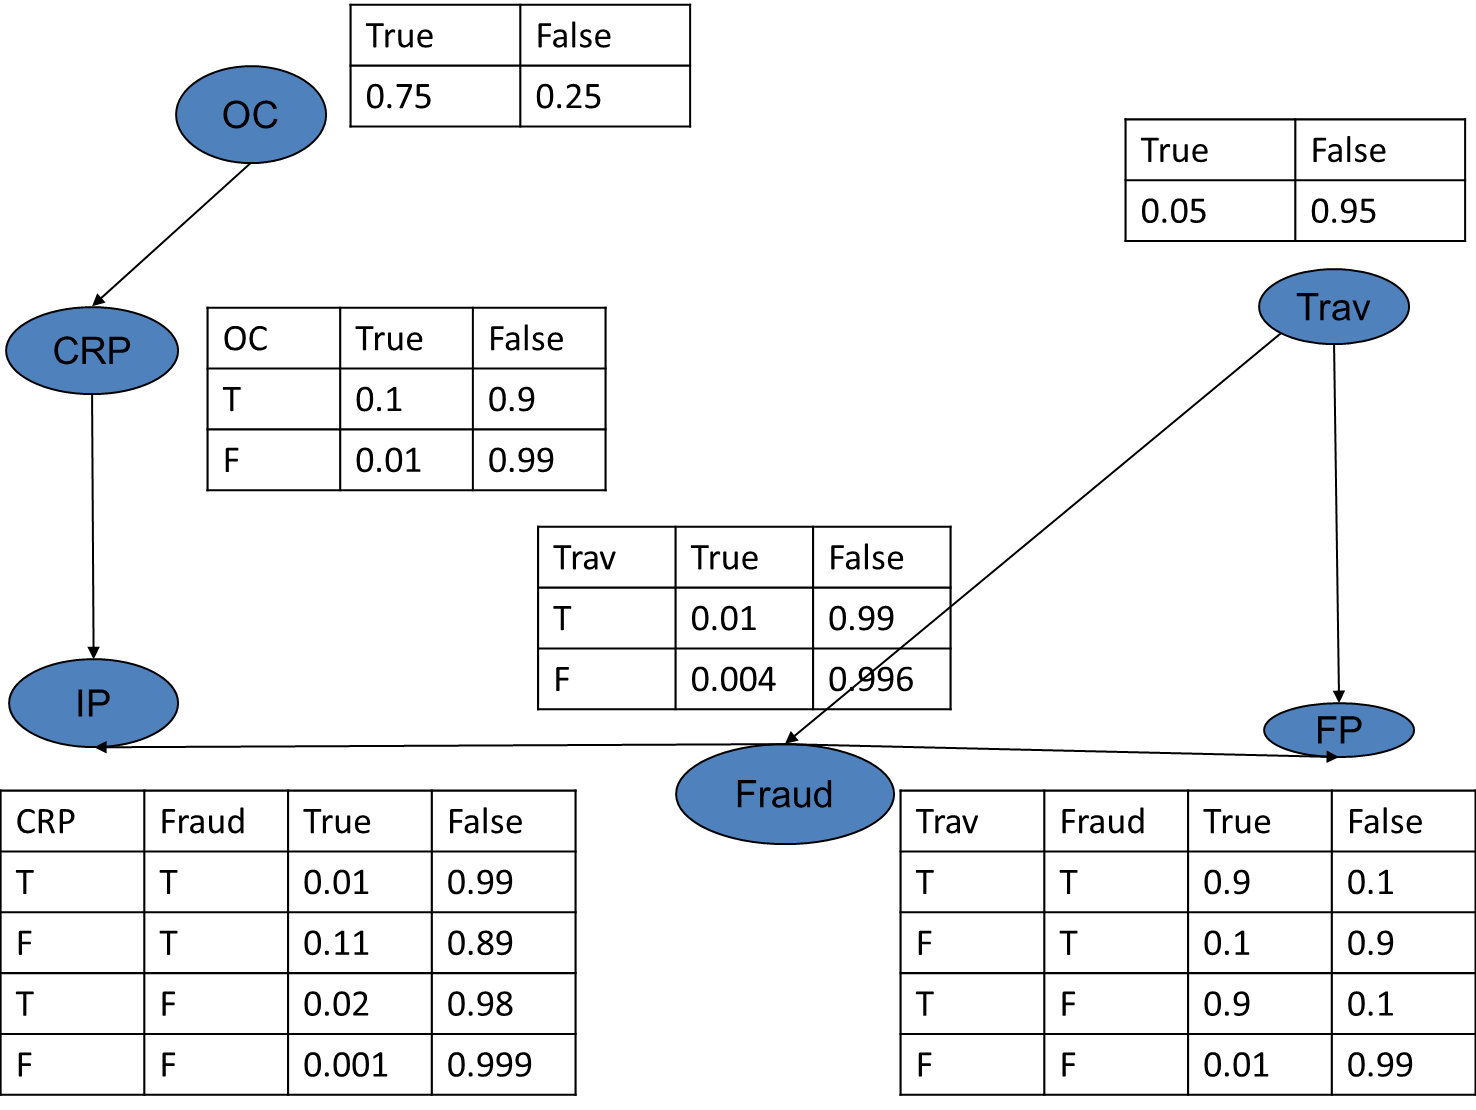
\includegraphics[width=1\textwidth]{fig/Picture1.png}
		\caption{Bayes Network to identify fraudulent transactions.}
		\label{fig:q3}
	\end{figure}

		     	 \begin{align*}
				 P(Fraud)
				 & = P(Fraud=T|Trav=T) * P(Trav =T) + P(Fraud=T|Trav=F) * P(Trav = F) \\
				 & = 0.01 * 0.05 + 0.004 * 0.95 \\
				 & =0.004275 \\
			 \end{align*}

Let the probability that the current transaction is a fraud once we have verified that it is a foreign
transaction, but not an internet purchase and that the card holder purchased computer related accessories
in the past week P!
			 \begin{align*}
				P(Fraud|FP)
				&=P(Fraud |Trav) P(FP|Trav,Fraud) P(Trav) +\\
				&+ P(Fraud|\neg Trav)P(FP|\neg Trav, Fraud)P(\neg Trav)\\
				&=0.01 *0.90 *0.05 + 0.004* 0.10* 0.95\\
				&=0.00045 + 0.00038\\
				&=0.00083\\
			\end{align*}
			 \begin{align*}
				P(Fraud|\neg IP,CRP, OC)
				&= P(\neg IP|CRP,Fraud) P(CRP) +\\
				&+ P(\neg IP|\neg CRP,Fraud)P(\neg CRP)\\
				&= P(\neg IP|CRP,Fraud)*\\
				&*(P(CRP|OC)*P(OC) + P(CRP|\neg OC)*P(\neg OC))+\\
				&+ P(\neg IP|\neg CRP,Fraud)*\\
				&*(P(\neg CRP|OC)*P(OC) + P(\neg CRP|\neg OC)*P(\neg OC))\\
				&=0.99*(0.1*0.75+0.01*0.25)+0.89*(0.9*0.75+0.99*0.25)\\
				&=0.99*0.02125+0.89*0.41625\\
				&=0.379\\
			\end{align*}
Answer. P = 0.379 * 0.00083 = 0.00031457
\end{problem}

\end{document}
